%% bare_jrnl.tex
%% V1.3
%% 2007/01/11
%% by Michael Shell
%% see http://www.michaelshell.org/
%% for current contact information.
%%
%% This is a skeleton file demonstrating the use of IEEEtran.cls
%% (requires IEEEtran.cls version 1.7 or later) with an IEEE journal paper.
%%
%% Support sites:
%% http://www.michaelshell.org/tex/ieeetran/
%% http://www.ctan.org/tex-archive/macros/latex/contrib/IEEEtran/
%% and
%% http://www.ieee.org/


\documentclass[conference]{IEEEtran}


\usepackage{graphics}
\usepackage{epsfig}
\usepackage{epstopdf}
\usepackage{theorem}
\usepackage{verbatim} % comentarios
\usepackage{amsmath}
\usepackage{algorithm}
\usepackage{algpseudocode}
\usepackage{mwe}
\usepackage{hyperref}
\usepackage{xspace}
\usepackage[export]{adjustbox}


\usepackage{array}
\newcolumntype{C}[1]{>{\centering\arraybackslash}p{#1}}

\newcommand{\etal}{\textit{et al.}\xspace}



% *** GRAPHICS RELATED PACKAGES ***
%
\ifCLASSINFOpdf
  % \usepackage[pdftex]{graphicx}
  % declare the path(s) where your graphic files are
  % \graphicspath{{../pdf/}{../jpeg/}}
  % and their extensions so you won't have to specify these with
  % every instance of \includegraphics
  % \DeclareGraphicsExtensions{.pdf,.jpeg,.png}
\else
  % or other class option (dvipsone, dvipdf, if not using dvips). graphicx
  % will default to the driver specified in the system graphics.cfg if no
  % driver is specified.
  % \usepackage[dvips]{graphicx}
  % declare the path(s) where your graphic files are
  % \graphicspath{{../eps/}}
  % and their extensions so you won't have to specify these with
  % every instance of \includegraphics
  % \DeclareGraphicsExtensions{.eps}
\fi
% graphicx was written by David Carlisle and Sebastian Rahtz. It is
% required if you want graphics, photos, etc. graphicx.sty is already
% installed on most LaTeX systems. The latest version and documentation can
% be obtained at: 
% http://www.ctan.org/tex-archive/macros/latex/required/graphics/
% Another good source of documentation is "Using Imported Graphics in
% LaTeX2e" by Keith Reckdahl which can be found as epslatex.ps or
% epslatex.pdf at: http://www.ctan.org/tex-archive/info/
%


% correct bad hyphenation here
\hyphenation{op-tical net-works semi-conduc-tor}

\IEEEoverridecommandlockouts

\begin{document}
%
% paper title
% can use linebreaks \\ within to get better formatting as desired
\title{An Empirical Study of Work Fragmentation in Software Evolution Tasks}
%
%
% author names and IEEE memberships
% note positions of commas and nonbreaking spaces ( ~ ) LaTeX will not break
% a structure at a ~ so this keeps an author's name from being broken across
% two lines.
% use \thanks{} to gain access to the first footnote area
% a separate \thanks must be used for each paragraph as LaTeX2e's \thanks
% was not built to handle multiple paragraphs
%

\author{
\IEEEauthorblockN{Heider Sanchez$^*$, Romain Robbes$^{\dagger}$} 
\IEEEauthorblockA{
Computer Science Department (DCC) \\
University of Chile, Chile
}

\and
\IEEEauthorblockN{Victor M. Gonzalez$^{\dagger}$}
\IEEEauthorblockA{Department of Computer Science \\ 
Instituto Tecnologico Autonomo de Mexico, Mexico}
\thanks{$^*$ supported by a research grant from CONICYT-Chile}
\thanks{$^{\dagger}$ supported by LACCIR Project RFP1212LAC004}
}



% make the title area
\maketitle


\begin{abstract}
%\boldmath
Information workers and software developers are exposed to work fragmentation, an interleaving of activities and interruptions during their normal work day. Small-scale observational studies have shown that this can be detrimental to their work. In this paper, we perform a large-scale study of this phenomenon for the particular case of software developers performing software evolution tasks. Our study is based on several thousands interaction traces collected by Mylyn, for dozens of developers. We observe that work fragmentation is correlated to lower observed productivity at both the macro level (for entire sessions), and at the micro level (around markers of work fragmentation); further, longer activity switches seem to strengthen the effect. These observations are basis for subsequent studies investigating the phenomenon of work fragmentation.
\end{abstract}


% Note that keywords are not normally used for peerreview papers.
\begin{IEEEkeywords}
Work fragmentation, interruptions, interaction data %empirical software engineering, mining software repositories
\end{IEEEkeywords}


% For peerreview papers, this IEEEtran command inserts a page break and
% creates the second title. It will be ignored for other modes.
\IEEEpeerreviewmaketitle




\section{Introduction}
% The very first letter is a 2 line initial drop letter followed
% by the rest of the first word in caps.
% 
% form to use if the first word consists of a single letter:
% \IEEEPARstart{A}{demo} file is ....
% 
% form to use if you need the single drop letter followed by
% normal text (unknown if ever used by IEEE):
% \IEEEPARstart{A}{}demo file is ....
% 
% Some journals put the first two words in caps:
% \IEEEPARstart{T}{his demo} file is ....
% 
% Here we have the typical use of a "T" for an initial drop letter
% and "HIS" in caps to complete the first word.

Work fragmentation is a phenomenon that has been extensively investigated in the literature. Several observational studies in company settings have shown that work fragmentation is very common in the workplace. These studies have also shown that work fragmentation is detrimental to the actual work taking place: after such a context switch, time is necessary for information workers to regain their bearings. A particularly harmful kind of work fragmentation is interruptions, where an external signal (email, chat, phone call, or direct conversation) forces an information worker to switch activity at an unplanned moment and for an unknown duration.

If the literature contains extensive studies of interaction workers, it lacks in two aspects: (1) most studies target information workers (fewer target the specific population of software developers), and (2) the studies are usually field studies, which are limited in the amount of data they contain.

Work fragmentation is indeed an important phenomenon within the context of modern software development, and the impact there may be even worse since developers build and maintain complex mental models of the software they are working on---these models may be more sensible to interruptions, and costly to rebuild. %; and 2) development is more often distributed, which may vary the nature of interruptions (trading high-bandwidth meetings for low-bandwidth electronic messages). Achieving flow in these conditions may be challenging.

In this paper, we present a study addressing these issues by (1) being focused on software developers, and (2) using MSR techniques to base its conclusions on a much larger amount of data (specifically, thousands of development sessions recorded by Mylyn). The downside is that the data exploited, being operational data \cite{M14}, is of lower quality than data extracted from a full-fledged observational study. Trading quality for quantity allows us to explore different aspects of the problem, and to generate hypotheses for subsequent studies of work fragmentation and interruptions in software development. We address the following three research questions:
\begin{itemize}
\item \textbf{RQ1:} What is the relationship between the observed interruptions and the observed developer productivity? 
\item \textbf{RQ2:} Is the observed relationship more pronounced in the presence of prolonged interruptions?
\item \textbf{RQ3:}  What is the observed relationship in the vicinity of interruptions?
\end{itemize}

\emph{A note on terminology}: in this paper we (ab)use the word \emph{interruption} to refer to a \emph{gap of activity} observed in IDE activity. We do not presume that all of these activity gaps are actual interruptions (our results lead us to believe otherwise); rather, we assume they are indicators of work fragmentation in general (that is, a programmer switching contexts to perform other activities while developing, such as answering email, looking for the solution of a problem on the Internet, etc). Of note, work by Zou and Godfrey \cite{ZG06} found that interruptions were a common cause for a lack of observed activity, and classified periods of inactivity as interruptions. %programmer feedback

\textbf{Structure of the paper.} We start with a literature review of studies of work fragmentation in Section 2. This section also contains a review of studies performed with the Mylyn dataset that we use. In Section 3, we describe the Mylyn dataset in further detail, highlighting potential issues in the operational data that we use in the analysis. In Section 4, we describe the measurements used in this study, and detail the processing of the data that is applied to alleviate the issues described in Section 3. The same section shows how we convert interaction traces to multivariate time series representing development sessions, and present the metrics in the analysis. In Section 5, we answer our first research question: we find an inverse relationship between number of interruptions and our three productivity indicators. In Section 6, we answer our second research question, finding that this relationship is more pronounced for development sessions with at least one longer interruption. Finally in Section 7 we answer our last research question and find that our productivity indicators are indeed lower in the vicinity of interruptions; we further find three patterns of interruptions with different characteristics. We close the paper by discussing the threats to validity of this study in Section 8, before concluding in Section 9.

%present the results of the study, first as a global analysis where the unit of study is the development session. We find that development sessions with indicators of work fragmentation have lower productivity than the ones who have not; further, longer switches away from development have a more pronounced effect, as was shown in other studies (ref victor). We also perform additional analysis at the finer-grained level of individual work fragmentation rather than whole sessions, finding that there are several categories of interruptions. In section 6, we detail the potential threats to validity of this study, before concluding in Section 7.

\section{Related Work}

\subsection{Empirical Studies of Work Fragmentation}

\paragraph{Studies of information workers}
In the modern workplace, people routinely multitask and shift their attention to multiple areas, projects and activities. An observational study by Gonzalez and Mark found that information workers experience high level of multitasking, averaging 3 minutes on a task before switching to another task \cite{GM04}. This often results in work fragmentation and interruptions which some studies found has detrimental effects to knowledge workers, such as stress and frustration \cite{MGK08}. Work fragmentation as result of interruptions usually demands extra effort to recover and resume pending activities: a study of 24 information workers found that a worker needs on average 25 minutes to get back on an interrupted task \cite{MGH05}. Similarly, Iqbal and Horvitz \cite{IH07} found that people experience disorientation and loss of context when multitasking. Czerwinsky \etal found that after experiencing work fragmentation people found it more difficult to perform interrupted tasks and took longer to complete them \cite{CHW04}. % Many other studies contribute either with anecdotical or experimental evidence of the detrimental effects of interruptions and work fragmentation. Most of them are based on retrospective assessment of the effects (not real time) by studies ́ subjects and without referring to aspects related to human cognitive activity such as attention, focus, or concentration.

While these studies already show the effect of work fragmentation is hurtful, they are mostly observational studies over a limited time, and do not address specifically the sub-population of programmers.

\paragraph{Studies specific to programmers}


%During their “Coding War Games” experiment [DeMarco 1985], where 166 programmers performed a day-long task in their usual working environment, they found that the most productive quartile of programmers experienced much less interruptions than the bottom quartile of programmers (according to surveys filled by the programmers).

Zou and Godfrey performed an analysis of interaction histories of 3 industrial programmers for a month \cite{ZG06}. One of their findings was the omnipresence of inactivity in the interaction data, that they interpreted as interruptions. They corroborated this with the programmers which agreed that many such periods of inactivity were indeed interruptions.

Similar to other information workers, software developers experience work fragmentation due to the nature of the activity. Ko et al. \cite{KDV07} performed an observational study of 17 Microsoft developers, where the average time before a switch was five minutes. Some switches were due to necessary changes between tasks, but others were
due to interruptions. 

Parning and Rugaber evidenced the presence of an edit lag in the majority of a large sample of development session spanning several datasets, hence showing that developers need time to resume work after an interruption~\cite{PR11}. Parnin and DeLine evaluated several cues  to help programmers resume work after interruptions forcing them to multitask~\cite{PD10}.

Maalej et al. \cite{MTRK14} performed a study on the program comprehension strategies of software developers. They found that developers often preferred direct interaction to consulting documentation. As such, experts on a piece of code were often interrupted in their work to answer questions from others.

Fritz et al. studied the perception developers have of their productivity. They found that developers perceived they were more productive on days where they accomplished significant tasks, and when they were not significantly interrupted \cite{MFMZ14}.

As above, most of these studies operate on small datasets. The study of Parnin and Rugaber is the closest to ours in terms of amount of data considered. However, the analysis performed on large datasets in their study focused principally on the edit lag metric, while we investigate metrics which are indicators of productivity along the entire session.


\subsection{Empirical Studies on Mylyn Data}

Several studies mining interaction data have been presented. Kersten and Murphy evaluated the effectiveness of their degree of interest (DOI) model by showing that in a field study of developers, users of their tools had a significantly higher edit to selection ratio \cite{KM06}. Fritz et al. evaluated how well DOI values reflected the developer’s knowledge of the code, and encountered mixed results \cite{FMH07}. The lessons they learned allowed them to develop a Degree of Knowledge (DOK) model, an extension of the DOI containing authorship information, and that was found useful in a variety of situations \cite{FOMM10}. The DOI has been implemented in Mylyn, and the data it generated has been used in several studies. Based on the data generated by an early version of Mylyn (which recorded additional data, namely usage of commands), Murphy et al. described how 41 Java developers used Eclipse, reporting on the most commonly used views and commands \cite{MKF06}

The Mylyn data available in the Eclipse issue tracking system was used in several studies. Ying and Robillard characterized the edit strategies of developers in the Mylyn dataset, finding three: edit-first, edit-last, and edit-throughout \cite{YR11}. Lee et al. developed Micro Interaction Metrics in order to enhance defect prediction models \cite{LJD11}. We investigated whether the duration of a task could be used to evaluate the accuracy of expertise metrics, with promising early results \cite{RD13}. Soh et al. studied the exploration patterns in the developer sessions of the Mylyn datasets, and classified their exploration strategies as referenced or unreferenced exploration; they find that unreferenced exploration were less time consuming \cite{SKGAA13}. Soh et al. conducted another study of this dataset, finding that the effort spent by a developer in a patch is not correlated with the implementation complexity of the patch \cite{SKGA13}. Bantelay et al. improved the accuracy of evolutionary couplings metrics for change prediction (usually computed with commit data); by adding interaction data, recall increased by 13\%, with a 2\% drop in precision \cite{BZK13}. Zanjani et al. integrated this approach with information retrieval techniques to support impact analysis based on textual descriptions of change requests \cite{ZSK14}.

% other interaction data
%Other studies were performed on additional datasets. Navtracks recommend source code files based on loops in the interaction data [Singer 2005], while DeLine et al. presented a similar approach, with the addition of sharing among a team [DeLine 2005]. Parnin et al. proposed to complement interaction histories with interaction logs, and showed initial results [Parnin 2005]. Later, Parning and Rugaber evidenced the presence of an edit lag in the majority of a large sample of development session spanning several datasets, hence showing that developers need time to resume work after an interruption [Parnin 2011]. They also evaluated several cues to help programmers resume work after interruptions forcing them to multitask [Parnin 2010].

%Coman and Silitti proposed an algorithm to identify tasks in development session [Coman 2009], that was evaluated with students performing tasks from Ko’s experiment [Ko 2006]. Zou and Godfrey found shortcomings in the algorithm in an industrial setting, with coarser tasks and longer development time [Zou 2012]. Earlier, Zou investigated whether programmers in an industrial study viewed files they do not change, and found that they were often more numerous than the ones that were changed [Zou 2006].

%Our studies of development sessions [Robbes 2007], code completion [Robbes 2008], interaction-based logical coupling [Robbes 2008], and change prediction [Robbes 2010] used a dataset of primarily change interaction data. Negara et al. also gathered a dataset of change interaction data, that was also augmented with test runs, refactorings, and SCM usage, and contrasted this data with data that would be recorded by an SCM system, showing the failings of the latter [Negara 2012]. Vakilian et al. recorded similar data, to specifically study the usage and usability of refactorings [Vakilian 2012]. Soetens et al. found that change interaction data was particularly well suited to detect refactorings in a preliminary study [Soetens 2013].

%Sahm and Maalej present Switch!, a tool that monitor interactions on the desktop in order to recommend a task context based on artifacts that are accessed together [Sahm 2010]. Roehm and Maalej monitor developer actions in order to detect their activities and difficulties, using Hidden Markov Models, with an initial precision of 72\% [Roehm 2012]. Carter and Dewan monitored user action in order to detect whether developers were having difficulties [Carter 2010].

%Yoon and Myers presented a tool, FLUORITE, that records low-level events from the Eclipse code editor [Yoon 2011]. They used data produced by FLUORITE to study 12 professional developers, and documented the various backtracking strategies they used, identifying various barriers to backtracking [Yoon 2012]. Yamashita performed studies of the impact of code smells in software development; the dataset included the interaction histories of several programmers, that were hired to work on the systems used in the experiment [Yamashita 2013]. Khodabandelou et al. applied intentional process mining techniques to the UDC dataset, devising algorithms to recover both intentions developers may have, and the low-level strategies they employed to achieve these intentions [Khodabandelou 2014]. 



%\begin{figure*}[!t]
%\centering
%\begin{tabular}{c}
%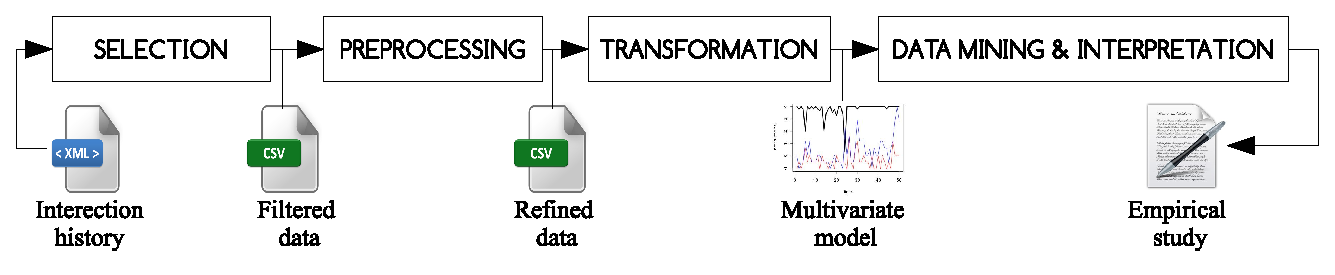
\includegraphics[width=0.9\linewidth,clip=,angle=0]{figures/phases} 
%\end{tabular}
%\caption{Schematization of phases involved in our study.}
%\label{fig:esq}
%\end{figure*}


\section{Data Description}

\subsection{Mylyn Data}
For our analysis, we used the Mylyn dataset of development data.  Mylyn \cite{KM06} is an Eclipe plugin that monitors the program elements a programmer interacts with in order to build a task context. A subset of Eclipse developers (principally from the Mylyn and PDE Eclipse projects) use the Mylyn Monitor tool to capture fine-grained usage data of their IDE that they attach to the bug fixes as a task context they submit to Eclipse. This allows reviewers of the bug fixes to use the same task context when they review the changes. The task context contains the entire interaction history since a developer activated the task he or she was working on, and as such is a rather reliable account of IDE usage over time (barring a few issues explained below).


To collect the data, we crawled the bugzilla data of the Eclipse project (\url{http://bugs.eclipse.org}), and downloaded all the bugs that had as an attachment a Mylyn task context.  In total, there were 6182 bug reports which contained 8102 Mylyn task contexts.


%\subsection{Bugzilla bug reports}
%Bugzilla is a Web-based tool for bug tracking and is installed as a plugin in Eclipse (\textit{http://bugzilla.org}).  This tool is used to organize and manager the solution of software defects and delegate responsibility to programmers. Bugzilla generates files XML call-bug reports, which maintain relevant information about the bugs that occurred.  The traces of interaction history are associated to each bug  report as an attachment.

\subsection{Interaction History Format}
The interaction history is a sequence of ordered events in time~\cite{YR11}.  An event is associated to a direct action of the programmer in program elements, for instance: edit and selection events. Other interaction events are indirect \cite{KM06}: they are issued by Mylyn itself while it is maintaining its DOI model of a programmer's task context. However these events are not edit or selection events. Each event captures several pieces of information: the timestamp, the kind of event and the signature of the code element that was interacted with (package, class, attribute, or method signature---including name and parameters). 

In Table \ref{tbl:kind_event} we show the different kinds of events and their description; in Table \ref{tbl:sample_event} we show an example of an interaction history. However, certain characteristics in the data present challenges around the data mining we plan to perform \cite{MFR14}. These cases must be detected and resolved in order to get a representative time series model of programmer activity. We describe these issues and our solutions below.


\begin{table}[ht!]
\renewcommand{\arraystretch}{1.3}
\caption{Kinds of interaction events~\cite{KM06}. }
\label{tbl:kind_event}
\centering
\begin{tabular}{|p{1.7cm}|p{1.3cm}|p{3.5cm}|} 
  \hline 
kind & mode & description \\  
  \hline 
    \hline 
selection & direct &  Editor and view selections via mouse \\
edit & direct & Textual and graphical edits  \\
command & direct & Operations such as saving, building, preference setting  \\
manipulation & direct & Direct manipulation of interest  \\
propagation & indirect & Interaction propagates to structurally related elements  \\
prediction & indirect & Capture of potential future interaction events \\
  \hline
\end{tabular}

\end{table}


\begin{table}[ht!]
\renewcommand{\arraystretch}{1.3}
\caption{ Example of interaction history. }
\label{tbl:sample_event}
\centering
\begin{tabular}{|c|l|c|c|c|} 
  \hline 
    & StartTime & EndTime & EventKind &  Method  \\
  \hline
  \hline
  1 & 10:30:00 & - & selection & m1  \\
  2 & 10:30:40 & - & manipulation & - \\
  3 & 10:30:40 & - & edit & m1  \\
  4 & 10:31:03.700 & - & selection & m1  \\
  5 & 10:31:03.800 & - & selection & m2  \\	  
  6 & 10:31:03.850 & - & selection & m3  \\	  
  7 & 10:32:05 & 10:33:07 & edit (5) & m2  \\	  
  8 & 10:33:10 & - & prediction & - \\
  \hline  
\end{tabular}
\end{table}


\subsection{Special Characteristics of Mylyn Data}
 Below, we describe the characteristics of Mylyn data one has to consider before processing them. This is especially relevant in our case since our study needs a representation of the activity as close to reality as possible.  In Section \ref{sec:trans} we describe the criteria used to process these characteristics. 


\textbf{Aggregate events. } This type of event includes several actions on the same program element. These actions usually occur within an interval of short duration time.  Whenever an aggregation occurs, the event is expanded to include two timestamps defining a range of time, instead of a single timestamp, and a number of events. Accordingly, these aggregate events lose their specific time besides the range of time. The reason of this is that for scalability---in terms of storage---Mylyn does not register all the user events.

For example, Table \ref{tbl:sample_event} shows an aggregate edit event in row 7. We indicate in parenthesis the number of actions associated and the field \textit{EndTime} registers the timestamp of the last occurrence. Clearly, too much aggregation in a given trace severely compromises the detection of work fragmentation as this relies on accurate timestamps.


\textbf{Massive events. } Such an event occurs when the same action is executed on more than one program element in a very short time. This massive action generates consecutive events of the same kind and with a tiny gap between them.

For example, massive events are produced when we select an entire group of classes from the navigation tree panel in Eclipse. In  Table \ref{tbl:sample_event} we show a massive selection on the methods m1, m2 and m3  in rows 4, 5 and 6. This massive selection produces three consecutive events with a time gap of not more than 0.1 seconds. These events overstate the activity of developers as each of these does not correspond to an individual developer action; rather, the entire sequence is.


\textbf{Very long events. } These events have a duration time ($|EndTime - StartTime|$) much larger than the mean. This mainly occurs in aggregate events. We believe that this issue is due to factors related to Mylyn, since it can register the end time of an event when the task is resumed after a long downtime. Another cause of these events is when one selects a code fragment and maintains this action for a long time. 
 
After exploring a sample of traces, we noticed that a long interruption of activity implicitly splits a trace into two sub-traces.  Moreover,  we have realized that many long events happen around this border. That is, they began before the interruption and finished immediately after the interruption, which confirms the observation above (resumption of a task after a long downtime). However this has the side effect of hiding the gaps of activity in the sequence of events if care is not taken. Consequently, the duration of these events is overstated; however, finding their actual duration is not trivial. 
%was extended beyond the significant real time, since it implicitly encapsulated  an interruption in its execution interval. 




\section{Preview Phases for Knowledge Discovery}
We used the phases of the process \textit{Knowledge Discovery in Databases (KDD~\cite{FPP96})} to discover useful knowledge from our collection of data: we first select data, then preprocess it, before transforming it to time series. We close this section by presenting the metrics we use in this study. %  (see Figure~\ref{fig:esq}). 

\subsection{Selection}
Our purpose is the analysis of work fragmentation and interruptions in software development. Therefore, we focused only in the interaction data of the user with the program elements. The  variables of interest for our study are~\cite{RD13}:
\begin{enumerate}
\item Duration: the time that a programmer took to perform a programming task. 
\item Edition:  the amount of code changes that were necessary to perform said task. %It is associated to the  edit events.
\item Navigation: how many program elements were consulted in a task; represented by selection events.
\item Edit ratio: as in previous studies \cite{KM06}, the ratio of edits over edits and selections is an indicator of more efficient work since program exploration is reduced.
\end{enumerate}

First, we have kept only the edit and selection events that are associated to a program element. These type of events are distributed in 8058 traces. On the other hand, edit-type events also occur when the programmer double clicks on a file. In these events the starting time and ending time are the same~\cite{LJD11}. We consider that the double-clicking actions form part of the user navigation, therefore these events are transformed into selection events.  

Second, we have kept all traces without aggregate information. Unfortunately, we cannot know the distribution in time of the actions that have been aggregated in a single event: without additional information, an aggregation of 15 events over one hour is as likely to have an event every 4 minutes than to have 10 events in the first 5 minutes and 5 more in the last 10 minutes. Therefore, designing a correct disaggregation task to this traces is very difficult, if not impossible.

In order to keep as many traces as possible, we have also kept a little group of traces with aggregate information where the aggregate events have a maximum duration time of five minutes (to minimize uncertainty) or have only two aggregate actions (since the actual event timestamps are known in this case). Thus, we were left with 6260 traces.

It could be possible that these traces we discarded were biased in one way or another. In Figure~\ref{fig:hist_rejected}, we note that in our data the traces with aggregation information appear from  the year 2008 on, and slowly increase in frequency from then. We would expect such a pattern from a change to the version of Mylyn, rather than a change to the type of tasks being performed. This is corroborated with our tests of a recent version of Mylyn, which seems to be even more aggressive in discarding information (it only keeps information at the class level, discarding method level information). As such, our assumption is that it is unlikely that this change is due to anything else than the version of Mylyn that was in use (and hence is not due to different tasks, people, etc). This leads us to believe that it is unlikely that filtering these traces would introduce other sources of bias.
 
%We assume the programmers used newer versions of Mylyn, which included the aggregation for grouping of collapsed events. Furthermore, 


\begin{figure}[!ht]
\centering
\begin{tabular}{c}
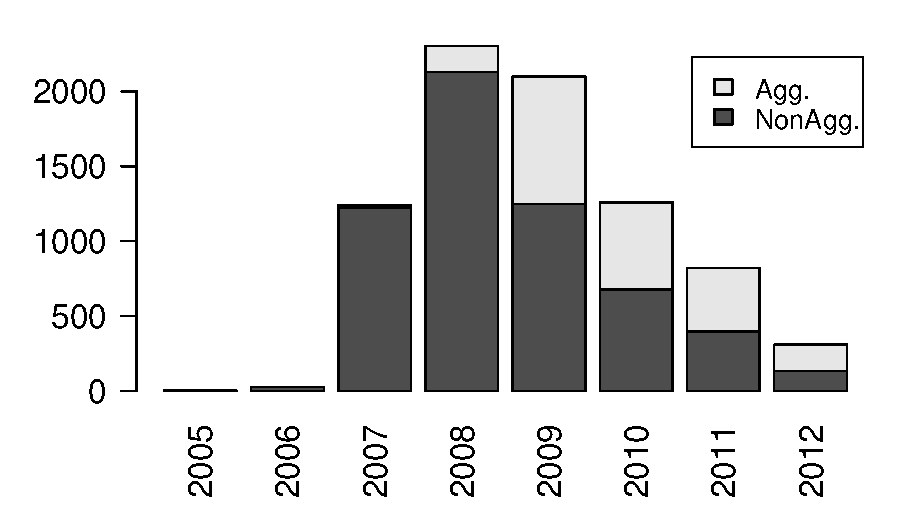
\includegraphics[width=1.0\linewidth,clip=, angle=0]{figures/hist_rejected} 
\end{tabular}
\caption{Grouping by date all the traces, with aggregate information (light gray) and without aggregate information (dark gray).}
\label{fig:hist_rejected}
\end{figure}

Finally, we found that 26\% of traces had at least an interruption over 8 hours, which is hence large enough to represent the difference between two working days. In these cases, we treated these long activity gaps as splitting points in order to decompose a long trace in several development sessions \cite{RL07}. 

After this, we considered a minimum duration time of 30 minutes in order to ensure a minimum of activity during a session. In this way, we obtained a final total of 4284 useful sessions to be processed in the next phase. 


\subsection{Preprocessing}\label{sec:trans}
After filtering out traces, we describe the final processing steps that yield the final development \emph{sessions} that we study:

\textbf{Sorting.} We sort chronologically all the events by their starting time. Before that, we normalize the timezone of each trace. We found 156 traces (3\%) with more than one timezone.  

\textbf{Massive events.} We use a short spacing interval to join consecutive massive events in only two, the first and the last event (Figure \ref{fig:mass_event}). We have considered a spacing size of 0.1 seconds (100 milliseconds). All the massive events we found were of type ``selection", which concurs which our observation above (multiple selection of several entities at the same time). The total number of selection events was reduced by 45\%.
% es una caracteristica mas comun de las selecciones, por lo tanto queremos minimizar el caso de edits. Con 0.1 logramos 

\begin{figure}[t]
\centering
\begin{tabular}{c}
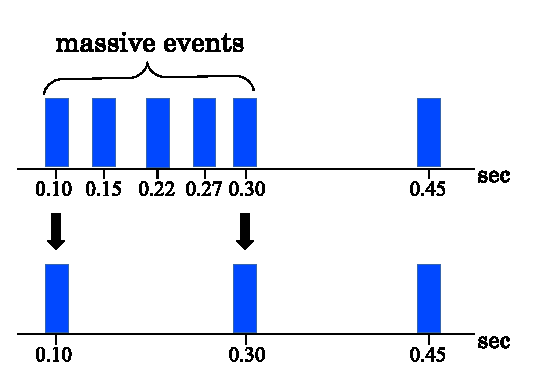
\includegraphics[width=0.75\linewidth,clip=, angle=0]{figures/mass_event} 
\end{tabular}
\caption{Replacing five massive events with only two events.}
\label{fig:mass_event}
\end{figure}

\textbf{Disaggregation.} We disaggregate all the actions associated with each remaining aggregate event with equidistant separation, as was done by Ying and Robillard \cite{YR11}. Due to the filtering above, this was only applied on traces that had aggregate events of short duration ($\leq$ 5 minutes).

\textbf{Event splitting.} Finally, we split all the long duration events. A normal event does not generally have duration (EndTime is null). However, 12\% of normal events  had a duration $> 0$ seconds and 3\% $\geq$ 1 hour, these events are outliers. Therefore, we split each long event in two events: one at the start and the other at the end of the interval. This is the same criteria applied for massive and aggregate events.

 Table \ref{tbl:mass_events} shows the ratio of variation of the number of events after preprocessing.
 
 \begin{table}[hb!]
 \renewcommand{\arraystretch}{1.3}
 \caption{Number of events after preprocessing.}
 \label{tbl:mass_events}
 \centering
 \begin{tabular}{l | c | c | c } 
   type event & before & after & \% variation  \\  
   \hline 
   edit &	 452236 & 475554 &	+5\%   \\
   selection &	658768 & 527652 & -20\%   \\
   \hline
   total & 1111004 & 1003206 & -10\%  \\
 \end{tabular}
 \end{table}

\subsection{Transformation}
Our goal is to build compact and representative models from each session. In this sense, we used aggregation of events to generate a multivariate time series (MTS). An MTS is a sequence of multivariate observations taken at continuous time intervals coming from a same phenomenon. We build the MTS with edit and navigation variables; the time unit is the minute, and the amplitude is the sum of all the events that occurred in this minute. We selected the minute as unit time because it seemed to be an appropriate and minimal representation of the user interaction in a programming task---obviously a subjective decision. 


Mylyn data has another characteristic which is unusual for time series: the time of occurrence of the events is not periodic (see column \textit{StartTime} in Table \ref{tbl:sample_event}). That is to say, events occur with non-equidistant separation gaps between them. However, in a time series, the values must be evenly spaced and chronologically sorted. For this reason, we compressed the size of the multivariate time series, pulling apart all the interruptions as a new time series variable. Then, each time series value represents the interruption duration in this minute (Figure \ref{fig:trans}). 


Consequently, the temporal component represents the \textit{real working time} of a programming task, excluding inactivity. This allows us to compute our activity indicators (number of edits, selections, edit ratio) independently of the amount of inactivity in a session.
% That is to say, each consecutive unit time corresponds to a minute of user activity, where there was at least one event of edit or selection. \\

We define empirically an interruption as a pause of programming of duration $\geq 3$ minutes. This is based on previous work where we observed that short interruptions lasted usually this long \cite{GM04}. Based on additional observations from this work, we defined a prolonged interruption as one lasting for more than 12 minutes. 

We identified that 98\% of sessions had at least one gap of activity. Moreover, we observe that the short interruptions predominate over the prolonged interruptions (Table \ref{tbl:by_duration}). This first result tells us that work fragmentation is extremely prevalent in our dataset.

\begin{table}[ht!]
\renewcommand{\arraystretch}{1.3}
\caption{prevalence of interruptions according to their duration time. }
\label{tbl:by_duration}
\centering
\begin{tabular}{p{2.1cm}|p{0.8cm}|p{3.4cm}} 
duration & ratio & examples  \\
  \hline   
$[3  - 12 min \rangle$ & 69\% & short pause, answer a question, thinking, looking for interruption  \\ 
\hline 
$[12  - 30 min \rangle$ & 18\% & coffee break, short meeting, extended interruption  \\
$[30 min - 2 hr \rangle$  & 9\% & lunch break, a meeting  \\
$[2 hr - 8 hr \rangle$ & 4\% & extended meeting \\
%$[8 hr - \infty \rangle$ & 0.14 & \textit{a long interruption}   \\
%$[8 hr -  \infty \rangle$ & 0.06  &  a weekend \\
%$[2 day - \infty \rangle$ & 0.04 & a long holiday \\ 
\end{tabular}
\end{table}

\subsection{Metrics Used in This Study}
We use the following six metrics to measure interruptions and productivity, while controlling for the unproductive time in a session, the length of time of the session itself, and the efficiency of the development that took place during the session:

Metrics characterizing interruptions:
	\begin{itemize}
	 \item \textit{Number of interruptions}:  counts all the interruptions that occur in a development session.
	 \item \textit{Duration of interruption}:  it is the time duration in minutes of the each interruption. 
	\end{itemize}

Metrics characterizing productivity and activity:
	\begin{itemize}
	 \item \textit{Productive work time:} the duration of a development session, substracting the duration of all the interruptions present in the session, to control for inactivity.
	 \item \textit{Number of edits per minute:} the total number of edits events, divided by the productive work time to control for length of the session. This is an indicator of user activity during the session.
	 \item \textit{Number of selections per minute:} is the total number of selection events, divided by the productive work time. Also an indicator of activity.
	 \item \textit{Edit ratio:} the number of edits divided by the sum of edits and selections, as used by Kersten and Murphy \cite{KM06}; an efficient developer spends less time exploring code and more time editing it.
	\end{itemize} 



%Completed this process, we obtained a set of multivariate time series models to be used in different mining tasks.


%After, we applied smoothing using local means to help us see a clearer signal (discover trends).

\begin{figure}[t]
\centering
\begin{tabular}{c}
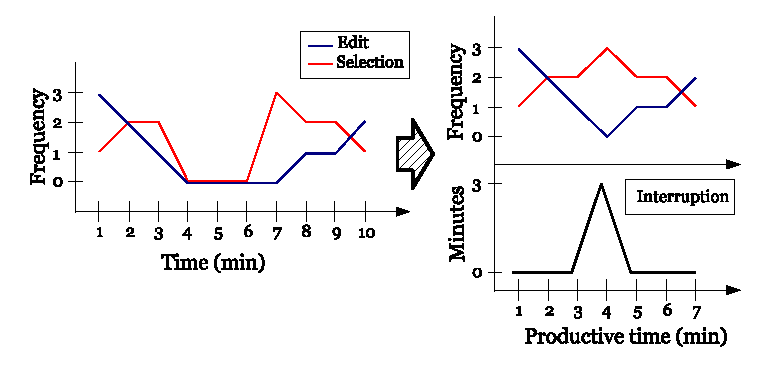
\includegraphics[width=.95\linewidth,clip=, angle=0]{figures/trans} 
\end{tabular}
\caption{Example of how to compress a time series. }
\label{fig:trans}
\end{figure}


%\section{Data Mining and Interpretation}
%In this section, we analyze the effect of the interruptions and work fragmentation in software development by means of exploratory and statistical analysis. To get a better view of the data, we first start by exploring the prevalence of interruptions and their relations with the productive time, before answering our research questions.

\section{RQ1: Relationship between Interruptions and Productivity}
%\subsection{Effect in the productive work time}

%In this section, we explore the relationship between interruptions and the productive time (that is, the time spent in a development session excluding interruptions). Figure \ref{fig:prod_int} is a scatterplot in which the x-axis indicates the number of interruptions and the y-axis indicates the productive work time; both are in logarithmic scale. The brown line emphasizes the lower limit in the relation of both variables: if a trace has $n$ interruptions, then, its minimum productive time is $n+1$ minutes. The graph shows that there is not a very significant relation between the number of interruptions and the productivity time.

%For instance, there are traces with a single interruption and  their productive time up to $2^8$ minutes ($\approx$ 4.3 hours). 

%\begin{figure}[!ht] \centering \begin{tabular}{c}
%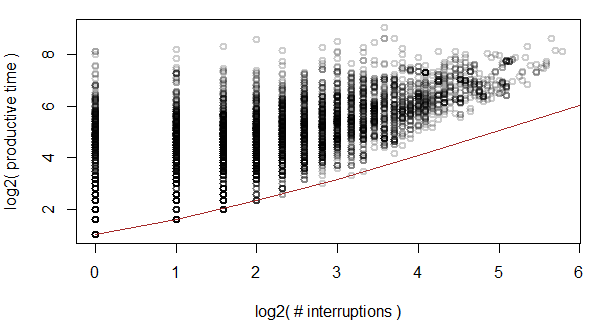
\includegraphics[width=.9\linewidth,clip=, angle=0]{figures/prod_int.png} 
%\end{tabular} \caption{Number of interruptions vs the productive work time. } \label{fig:prod_int} \end{figure} 

%In the second scatter plot, we plot the total duration of the in the x-axis and the productive time on the y-axis (Figure \ref{fig:prod_dura}). We observe a higher average of productive time in traces that had a lesser amount of interruptions. For instance, the traces that have accumulated $\leq 16$ minutes in interruptions, their productive time was $\geq 15$ minutes. Then, according as the duration increases, traces with a lower productive time were appearing. Thus, for example, we found 73 traces that had one interruption $\geq 28$ minutes but only two minutes of productive time. Therefore, we can appreciate a slight effect of long interruption duration over the productive time of the traces. 

%\begin{figure}[!ht] \centering \begin{tabular}{c}
%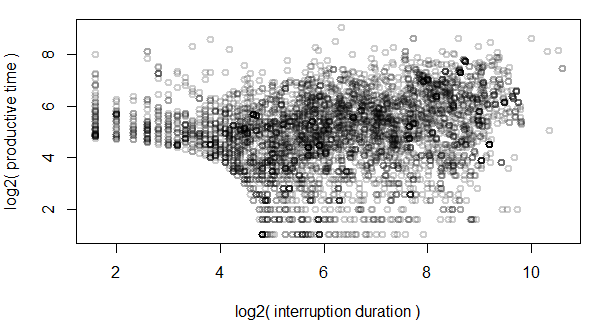
\includegraphics[width=.9\linewidth,clip=, angle=0]{figures/prod_dura.png} 
%\end{tabular} \caption{Total duration of interruptions vs the productive work time.. } \label{fig:prod_dura} \end{figure}



\subsection{Relation between Interruptions, and Edits and Selections}

As mentioned above, we use the metrics of edit, selection, and edit ratio as indicators of productivity. We first examine the number of edits and selections, and how their distribution varies in function of the number and type of interruptions.
 %we assume that the productivity is in function of the number of edit and selection events that the programmer performs in a trace. 

%First, we analyzed the number of interruptions over the productivity. In this sense, 
We split the data in five groups: The first group contain all the sessions without interruptions (\textit{none}). For the others groups, we have considered four ranges of number of interruptions delimited by their quartiles (Table \ref{tbl:quartil_int}). Then, for each group, we display the distribution of events per minute and edit ratio via boxplots (Figure \ref{fig:box_int_events}). We observe a large difference between the sessions without interruptions and the ones who do. Further, we observe that the rate of events per minute decreases slightly when the session has more interruptions. Therefore, we can intuit that the relationship between number of interruptions and the productivity indicators that are edits and selections, tends to be inversely proportional. 

\begin{table}[ht!]
\renewcommand{\arraystretch}{1.3}
\caption{Thresholds used to group sessions based on their number of interruptions} %separate the data in four percentages groups regarding the number of interruptions in each trace.}
\label{tbl:quartil_int}
\centering
\begin{tabular}{l | p{0.6cm} | p{0.6cm} | p{0.6cm}} 
     & $25\%$ & $50\%$ & $75\%$ \\  
  \hline 
  quartile &  3 & 5 & 10  \\   
\end{tabular}
\end{table}



\begin{figure}[!ht]
\centering
\begin{tabular}{c}
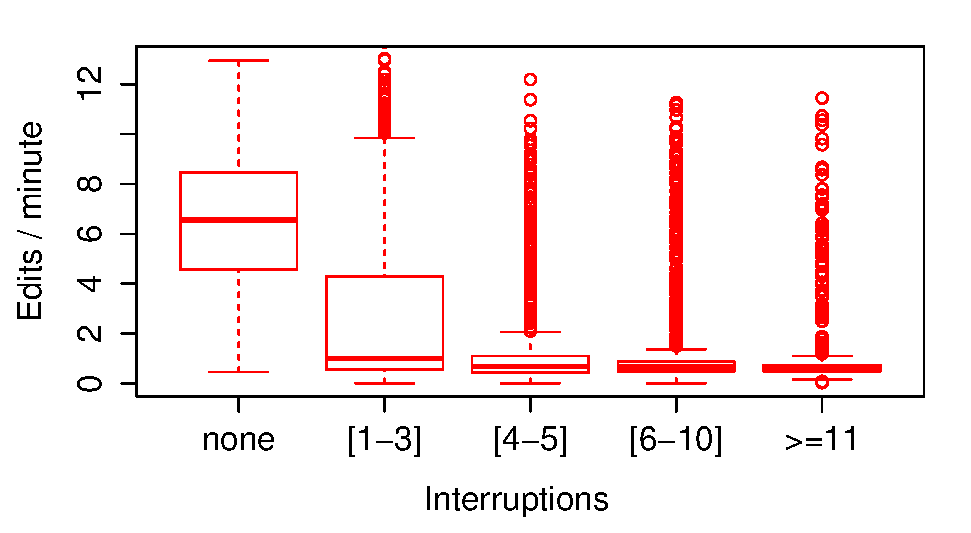
\includegraphics[width=.8\linewidth,clip=, angle=0]{figures/box_int_events_edit}  \\
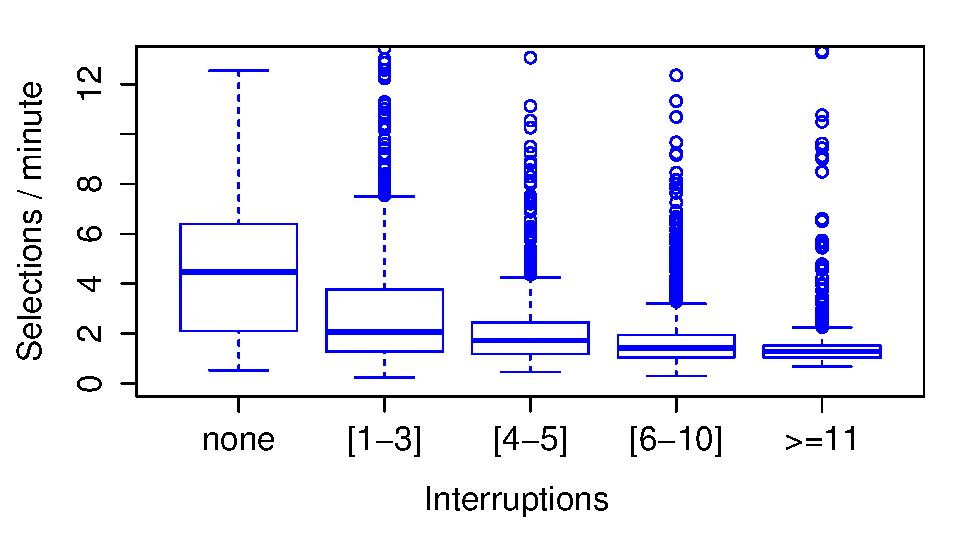
\includegraphics[width=.8\linewidth,clip=, angle=0]{figures/box_int_events_sel}  \\
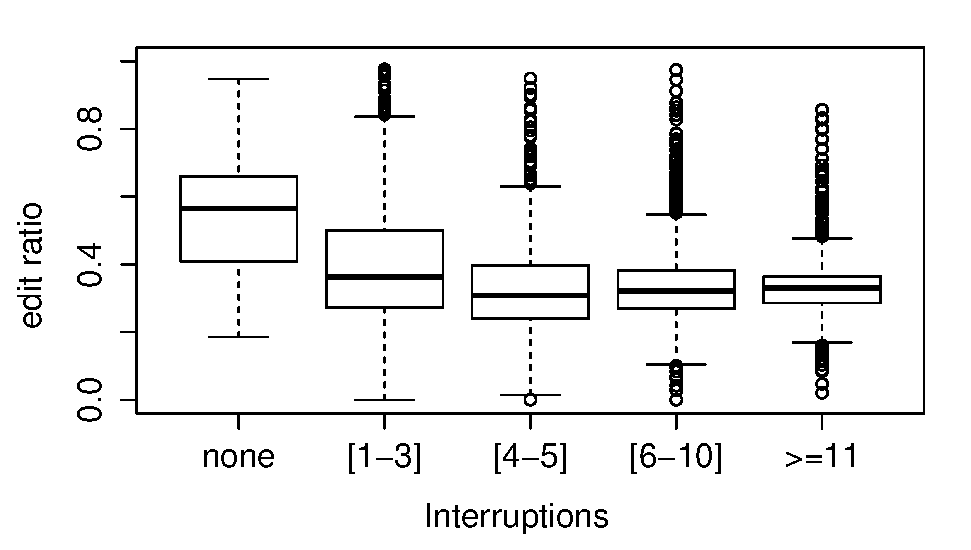
\includegraphics[width=.8\linewidth,clip=, angle=0]{figures/box_int_ratio} \\
\end{tabular}
\caption{Boxplots showing the relation between the number of edits and selection events per minute, the edit ratio, and the number of interruptions. }
\label{fig:box_int_events}
\end{figure}

Beyond visual inspection, we also quantify the statistical and the practical significance of these observations. First, all the differences observed are statistically significant with very low p-values (see Table~\ref{tbl:p_value}) according to the Mann-Whitney U-test. This is not surprising, given the shape of the boxplots and the size of the samples.

More importantly, we used \textit{Cohen's d} to measure the practical significance of these results in term of effect size % the effect size of the differences in means as standardized difference~
\cite{C94}. \textit{Cohen's thresholds} are defined as follows: trivial ($<0.2$), small  ($\langle 0.2 - 0.5 ]$), moderate ($\langle 0.5 - 0.8 ]$) and large effect ($> 0.8$). As shown in Table \ref{tbl:p_value}, we note that the effect size of the interruptions over the number of edits by minute is (very) large. In selections, the effect is moderate for sessions having up three interruptions, and large to very large for sessions with over four interruptions. This reinforces our impressions that interruptions and user activity follow inverse relationships, and that they are quite pronounced.

%We conclude that the user productivity could be adversely affected by increased interruptions.

\begin{table}[ht!]
\renewcommand{\arraystretch}{1.3}
\caption{Effect size and significance of the relationship between number of edit per minute, selection per minute, edit ratio, and number of interruptions} 
\label{tbl:p_value}
\centering
\begin{tabular}{l | C{0.75cm} | C{0.85cm} | C{0.85cm} | C{0.85cm} |p{0.75cm}} 

   & none & $\leq 3$ & $[4 - 5]$ & $[6 - 10]$ & $\geq 11$  \\  
  \hline
  \multicolumn{6}{c}{\textbf{Edits}} \\
  \hline
  mean & 6.29 &	2.59 & 1.55 & 1.29 & 0.91  \\ 
  % \cline{3-6} 
  %t.test & $\hookrightarrow$& \multicolumn{4}{c}{$<$ 2.2e-16} \\
   \cline{3-6} 
  U-test & $\hookrightarrow$ & \multicolumn{4}{c}{$<$ 2.2e-16} \\
  \cline{3-6} 
  Cohen's $d$ & $\hookrightarrow$	& \textbf{1.23} & \textbf{2.02} & \textbf{2.37} & \textbf{3.31}    \\
  \hline
  
  
  \multicolumn{6}{c}{\textbf{Selections}} \\
  \hline 
  mean & 4.73 &	2.93 & 2.26 & 1.79 & 1.54  \\ 
    % \cline{3-6} 
    %t.test & $\hookrightarrow$& 6.258e-08 & 1.623e-12 & 4.87e-16 & $<$ 2.2e-16 \\
     \cline{3-6} 
    U-test & $\hookrightarrow$ & 8.1e-13 & \multicolumn{3}{c}{$<$ 2.2e-16} \\
    
  \cline{3-6} 
  Cohen's $d$ & $\hookrightarrow$	& \textbf{0.66} & \textbf{1.17} & \textbf{1.93} & \textbf{1.78} \\  
\hline


  \multicolumn{6}{c}{\textbf{Edit ratio}} \\
  \hline 
  mean & 0.55 & 0.39 & 0.33 & 0.34 & 0.33 \\ 
  \cline{3-6} 
%    t.test & $\hookrightarrow$& 1.62E-13 & \multicolumn{3}{c}{$<$ 2.2e-16} \\
     \cline{3-6} 
    U-test & $\hookrightarrow$ & 4.2e-14 & \multicolumn{3}{c}{$<$ 2.2e-16} \\
    \cline{3-6} 
    Cohen's $d$ & $\hookrightarrow$ & \textbf{0.84} & \textit{1.33} & \textit{1.48} & \textit{2.12} \\ 
\hline

\end{tabular}
\end{table}

\subsection{Effect on the Edit Ratio}
Finally, we want to know the effect the interruptions over the ratio of edits in each session, as this is the often seen as a better indicator of productivity than raw activity, since the programmer spends less time navigating the source code in search of information, and more time actively editing it \cite{KM06}.

We first analyze the relationship between edit ratio and number of interruptions (Figure \ref{fig:box_int_events}, bottom). We observe that the edit ratio decreases when the session has more interruptions: the effect is pronounced between session that do not have interruptions and ones that do, and is more subtle as the number of interruption grows. A look at the practical and statistical significance of these results (Table \ref{tbl:p_value}, bottom) show that the results are (unsurprisingly) statistically significant, and that the observed effect sizes are large to very large.

Adding this to our previous result, we observe that both the user activity (in terms of raw quantity of edits and selections per minute) and the user productivity (in terms of edit ratio), both follow an inverse relationship with the number of interruptions. This finding agrees with the previous literature on the harmfulness of multitasking, work fragmentation, and interruptions. Furthermore, the effect sizes are very large.

%\begin{table}[ht!] \renewcommand{\arraystretch}{1.3} \caption{effect size of relationship between number of interruptions and ratio of edition.} \label{tbl:test_ratio1} \centering
%\begin{tabular}{l | C{0.7cm} | C{0.75cm} | C{0.84cm} | C{0.99cm} |p{0.75cm}}
%   & none & $\leq 3$ & $[4 - 5]$ & $[6 - 10]$ & $\geq 11$  \\  
%  \hline
%  mean & 0.55 & 0.39 & 0.33 & 0.34 & 0.33 \\ 
%  \cline{3-6} 
%    t.test & $\hookrightarrow$& 1.62E-13 & \multicolumn{3}{c}{$<$ 2.2e-16} \\
%     \cline{3-6} 
%    wilcox & $\hookrightarrow$ & 4.21E-14 & \multicolumn{3}{c}{$<$ 2.2e-16} \\
%    \cline{3-6} 
%   effect size & $\hookrightarrow$ & \textbf{0.84} & \textit{1.33} & \textit{1.48} & \textit{2.12} \\ 
%\end{tabular}
%\end{table}

\section{RQ2: Relationship between Duration of Interruptions and Productivity}

In this section we analyze whether or not the interruption duration is a factor in the relationship between interruptions and developer productivity. To substantiate this claim, we have built two groups of sessions with interruptions:
\begin{itemize}
\item \textit{short}: the first group consists of sessions that only have short interruptions ($<$ 12 minutes of duration). These sessions constitute 18\% of the total.
\item \textit{prolonged}: the second group consists of the remaining sessions, which have at least one prolonged interruption ($\geq$ 12 minutes of duration). These session constitute 80\% of the total.
\end{itemize} 

We then displayed the distribution of events by minutes and edit ratio of these two groups and compared them with the sessions without interruptions (Figure \ref{fig:box_dur_events}). We observe that the number of events per minute is lower in sessions with at least one prolonged interruption. 

As in the previous case, the differences are significant, and we used \textit{Cohen's d} to measure the practical significance of the means (Table \ref{tbl:p_value2}). We note that the effect size of the interruption duration over the number of edits per minute is very large. In selections, the effect is moderate for short interruptions, and large for prolonged interruptions. We conclude that the relationship between user activity and interruptions could be adversely affected by interruptions of longer duration. 

\begin{figure}[!ht]
\centering
\begin{tabular}{c}
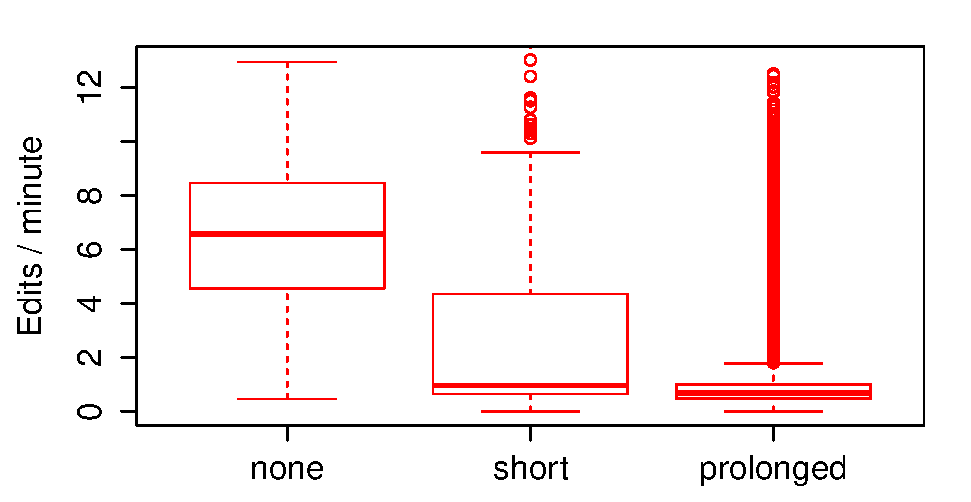
\includegraphics[width=.8\linewidth,clip=, angle=0]{figures/box_plot_range_edit}  \\
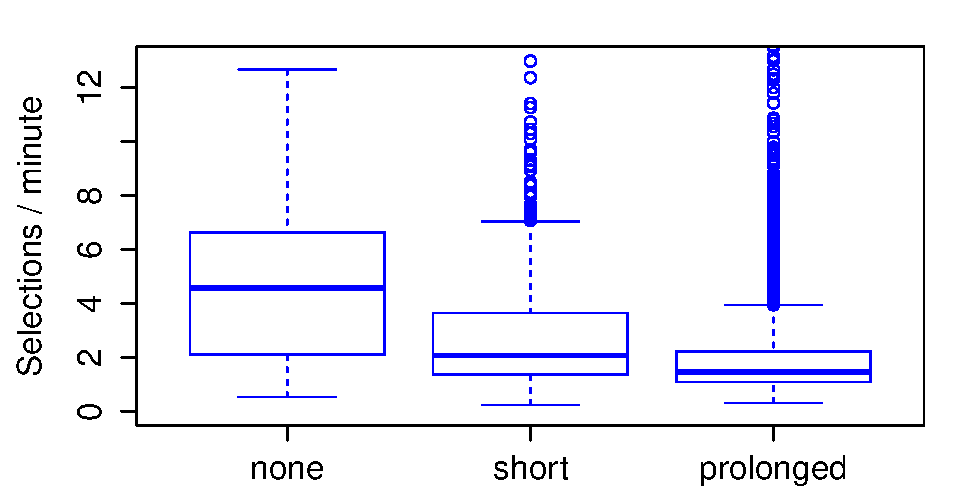
\includegraphics[width=.8\linewidth,clip=, angle=0]{figures/box_plot_range_sel}  \\
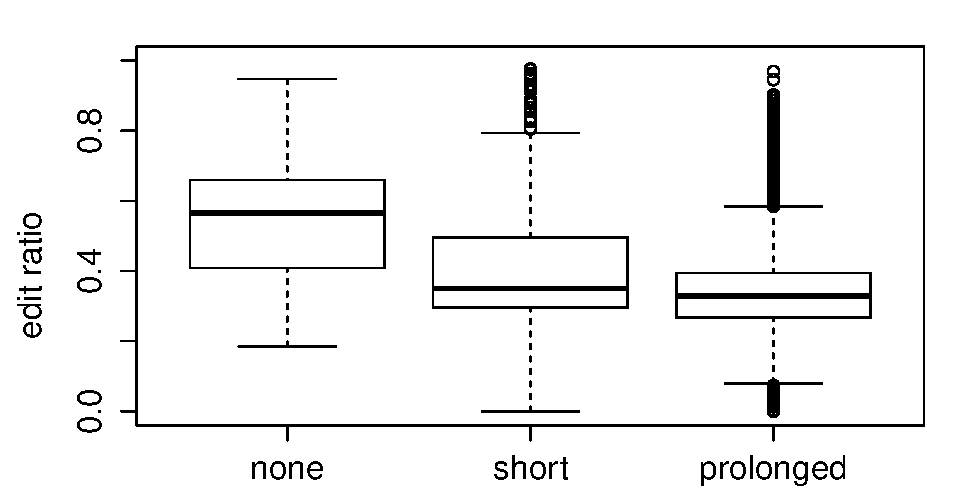
\includegraphics[width=.8\linewidth,clip=, angle=0]{figures/box_dur_ratio}
\end{tabular}
\caption{Boxplots showing the relation between the number of edits and selections per minute, the edit ratio and interruption duration}
\label{fig:box_dur_events}
\end{figure}

%\begin{figure}[!ht]
%\centering
%\begin{tabular}{c}
%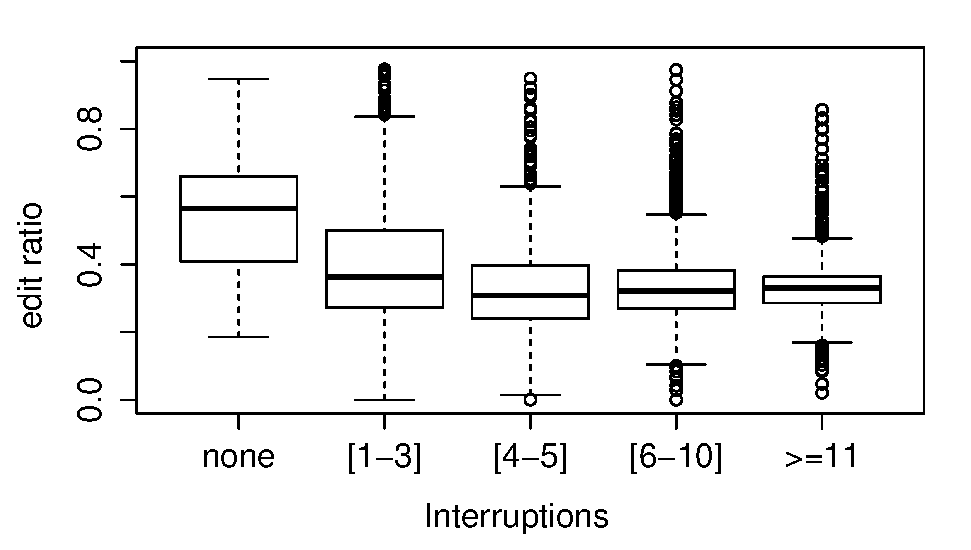
\includegraphics[width=.8\linewidth,clip=, angle=0]{figures/box_int_ratio} \\
%\end{tabular}
%\caption{Boxplots of traces for showing the ratio of editions compared to the number of interruptions (top) and to the interruption duration (bottom). }
%\label{fig:box_ratio}
%\end{figure}



\begin{table}[ht!]
\renewcommand{\arraystretch}{1.3}
\caption{Effect size and statistical significance of the relationships between edits and selection per minute, edit ratio, and duration of interruptions} %, and editions and selections.}
\label{tbl:p_value2}
\centering
\begin{tabular}{l | p{0.7cm} | C{1.9cm} | C{1.9cm} } 
   & none & short &  prolonged  \\  
  \hline
  \multicolumn{4}{c}{\textbf{Edits}} \\
  \hline
  mean & 6.96 &	2.98 & 1.76 \\ 
  % \cline{3-4} 
  %t.test & $\hookrightarrow$& \multicolumn{2}{c}{$<$ 2.2e-16} \\
   \cline{3-4} 
  U-test & $\hookrightarrow$ & \multicolumn{2}{c}{$<$ 2.2e-16}  \\

  \cline{3-4} 
  Cohen's $d$ & $\hookrightarrow$	& \textbf{1.23} & \textbf{2.11}   \\
  \hline
  
  
  \multicolumn{4}{c}{\textbf{Selections}} \\
  \hline 
  mean & 5.20 &	3.33 & 2.47 \\ 
  % \cline{3-4} 
  %t.test & $\hookrightarrow$& 2.089e-08 & 8.175e-14 \\
   \cline{3-4} 
  U-test & $\hookrightarrow$ & 6.197e-13 & $<$ 2.2e-16 \\
  
  \cline{3-4} 
  Cohen's $d$ & $\hookrightarrow$	& \textbf{0.63} & \textbf{1.24}  \\  
  \hline
  \multicolumn{4}{c}{\textbf{Edit ratio}} \\
  \hline 
  mean & 0.55 & 0.40 & 0.34\\ 
%   \cline{3-4} 
%  t.test & $\hookrightarrow$&  4.20E-12 & $<$ 2.2e-16 \\
   \cline{3-4} 
  U-test & $\hookrightarrow$ & 3.72e-14 & $<$ 2.2e-16  \\
  \cline{3-4} 
  Cohen's $d$ & $\hookrightarrow$ & \textit{0.86} & \textit{1.32}\\
\hline

\end{tabular}
\end{table}

%\begin{table}[ht!] \renewcommand{\arraystretch}{1.3} \caption{Effect size of the relationship between duration of interruptions and  ratio of edition.} \label{tbl:test_ratio2} \centering
%\begin{tabular}{l | p{0.7cm} | C{1.9cm} | C{1.9cm} } 
%   & none & short &  prolonged  \\  
%  \hline
%  \multicolumn{4}{c}{\textbf{Edits}} \\
%  \hline
%  mean & 0.55 & 0.40 & 0.34\\ 
%   \cline{3-4} 
%  t.test & $\hookrightarrow$&  4.20E-12 & $<$ 2.2e-16 \\
%   \cline{3-4} 
%  wilcox & $\hookrightarrow$ & 3.72E-14 & $<$ 2.2e-16  \\
%  \cline{3-4} 
%  effect size & $\hookrightarrow$ & \textit{0.86} & \textit{1.32}\\
%\end{tabular} \end{table}



Similar results occurs when we look at the edit ratio (Figure \ref{fig:box_dur_events}, bottom): the edit ratio is smaller in sessions that have prolonged interruptions, compared to the ones that only have short interruptions. At the bottom of Table \ref{tbl:p_value2}, we show the statistical and practical significance of these results. As before, we observe large effect sizes when comparing sessions who do not have interruptions with ones that do have, and larger effect sizes for sessions with at least one longer interruption.

These findings seem to indicate that the inverse relationship between productivity and time of duration is more pronounced in session with at least one longer interruption. This agrees with the literature for information workers.

\section{RQ3: Local Relationships between Interruptions and Productivity}

\subsection{Generic Sessions}
In order to better understand the relationship between work fragmentation and productivity, we need to delve deeper and perform local analyses of the development sessions. In the first step, we wanted to summarize how the activity of users is distributed over time in sessions which have no interruptions, short interruptions, and prolonged interruptions. 

To summarize the development sessions, we have resized each time series to a single $size$, using local means. We have used $size = 10$, that is, dividing each session in 10 chunks of equal time, since because it yielded better global visualization (better uniformity) of the user interaction along a session. For each chunk, we choose the median value of edits and selections for each group, and compose one summary time series for each group; these are the time series displayed in Figure \ref{fig:bins_int}.

We observe that the median activity in sessions with interruptions is less than in sessions without interruptions, mainly in the edit frequency. Moreover, the edit frequency exceeds the selection frequency in sessions without interruptions. The opposite occurs in sessions with at least one interruption---and is more pronounced when there is at least one prolonged interruption---, where the code navigation tends to exceed the frequency of edits. These results agree with our earlier results. 

We also notice that the time series without interruptions have much more edits in the middle of the session than the others. This observation matches the hypothesis that developers need time to build their mental model for their task, and are less productive early in a session. This is similar to the edit lag in Parnin's study~\cite{PR11}: in sessions without interruptions, the edit lag is clearly visible at the start of the session. This behavior is not visible in sessions with interruptions; indeed, each session may have several edit lags (after each interruptions), and those would be equally distributed over the entire duration of the session, resulting in the ``flat lines" that we see for these sessions.



These results support our previous observations at a finer level, an corroborate the literature saying that time is needed to start or get back on task.

%Therefore, with this result, we also infer that the presence of interruptions in a programming task could reduce the user interaction with the program. \\

%Another way to understand the effect of the interruptions in a programming task, was building global representations of the user activity e have considered three global representations for three groups of traces: the first trace represents to the traces without interruptions, the second to the traces that only  have short interruptions and the third to the traces that have at less one prolonged interruption. Then, 

\begin{figure}[!ht]
\centering
\begin{tabular}{c}
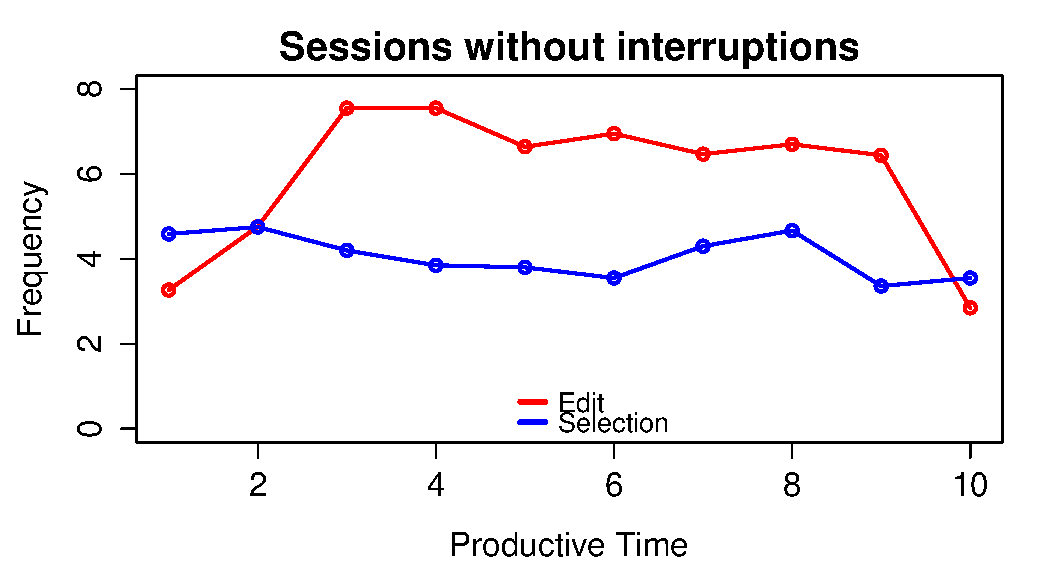
\includegraphics[width=.80\linewidth,clip=, angle=0]{figures/without_int_med} \\
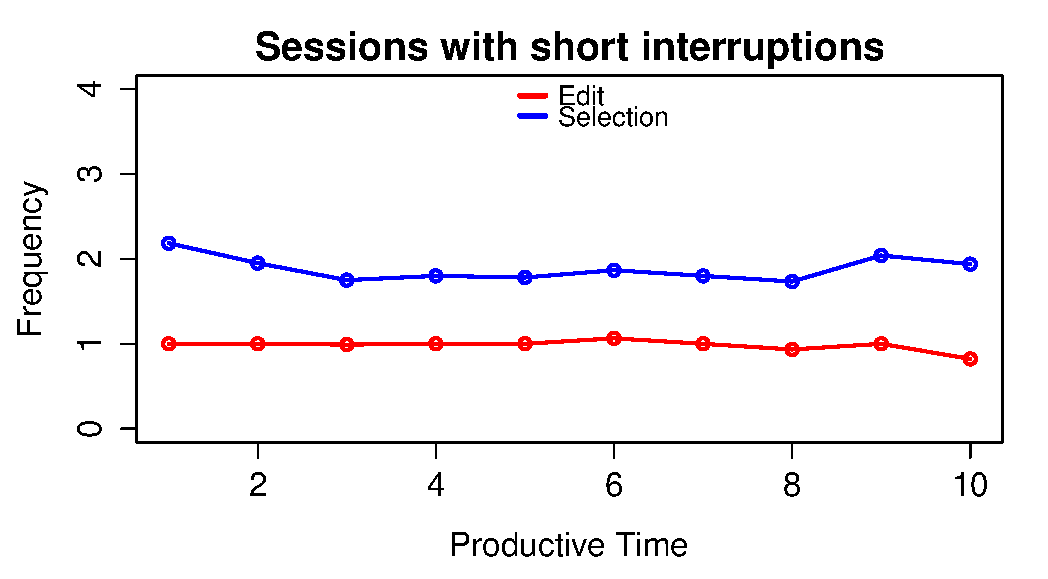
\includegraphics[width=.80\linewidth,clip=, angle=0]{figures/with_int1_med} \\
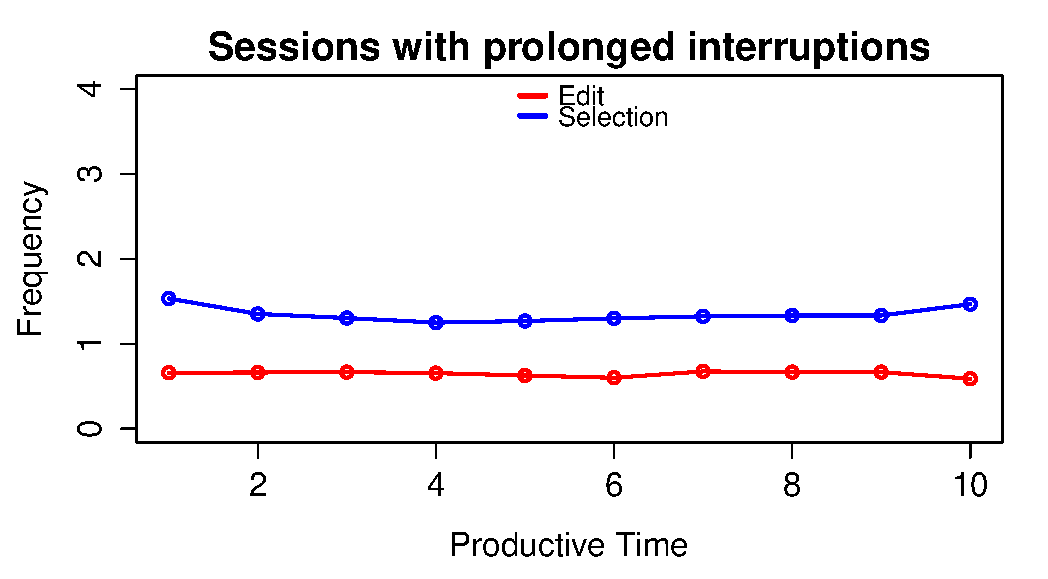
\includegraphics[width=.80\linewidth,clip=, angle=0]{figures/with_int2_med} 
\end{tabular}
\caption{Global representation of a session with: no interruptions (top); only short interruptions (middle); and at least one prolonged interruption (bottom). }
\label{fig:bins_int}
\end{figure}


\subsection{Local Analysis}
Having presented the global effect of the interruptions over the user productivity, we now focus on the local activity before and after interruptions. We take a maximum real time interval of 30 minutes around each detected interruption, obtaining a set of 26988 time series subsequences. Then, we compute the median of all these subsequences as a generic local representation (Figure \ref{fig:all_ints}). We also plot with dashed lines the median values of edits and selections per minute in the sessions with interruptions in order to give more context to the observed values.
%where another interruption  should not have been found. 
Below we describe some observations:
\begin{itemize}
\item \textit{In the center,} we find the interruption point. There is clearly a negative effect on the time series, as the area before and after the interruption is the area with the lowest activity. The activity is well below the median activity of time series with interruptions, showing that the effect is indeed more pronounced near interruptions.

\item \textit{On the right,} the trend of the time series increases steadily. We hypothesize that the programmer is immersing again into the programming task, increasing progressively the activity as represented by the number of edits and selections. We see that in the average case, it reaches the median activity 12 to 18 minutes after the interruption. It then rises further than the session median, which is not surprising, as we expect higher than median activity further away from interruptions.

%We called \textit{recuperation time} the first intersect point between edition and navigation. In this sense, the  average recuperation time of an interruption occurs in the minute 12. 

\item \textit{On the left,} we observe that the number of events near the interruption also goes down well below the median value. This is because work fragmentation is not only due to interruptions: programmers may for instance switch away from the IDE to look up information on the web or request it from other programmers. They are likely to do so because they are stuck, which would manifest itself by lower activity before the activity gap. We investigate this further below.

%This is more surprising, as we expected the activity to drop mostly after the interruption rather than before. A possible explanation is that their are several causes for inactivity
\end{itemize}


\begin{figure}[!ht]
\centering
\begin{tabular}{c}
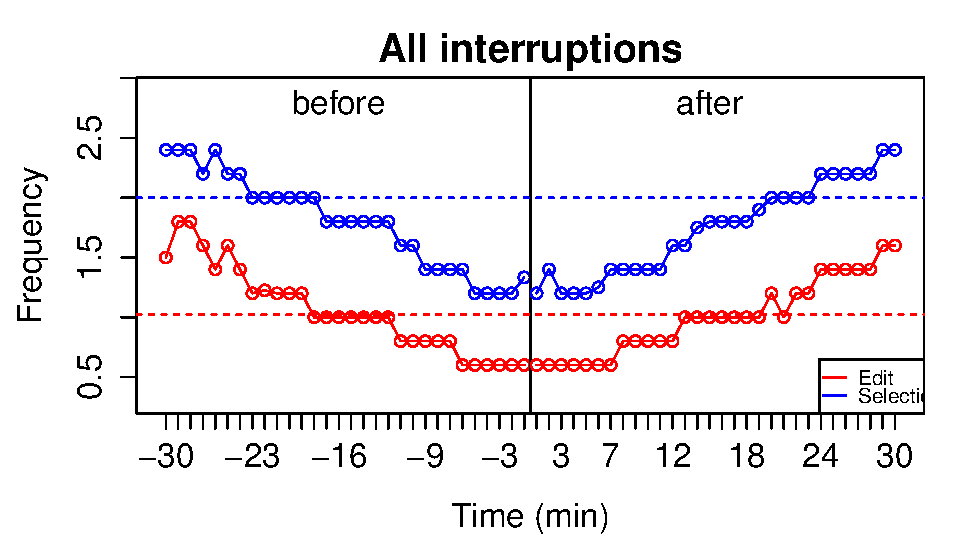
\includegraphics[width=0.9\linewidth,clip=, angle=0]{figures/all_ints} 
\end{tabular}
\caption{Local effect of an interruption in the user activity.}
\label{fig:all_ints}
\end{figure}


We investigated whether the drop in activity local to interruptions was also accompanied by a drop in the edit ratio. We computed the edit ratio over slices of 5 minutes before and after each interruption (smaller intervals would be too sensitive to noise). The boxplots in Figure \ref{fig:ratio_all} show that the edit ratio drops slightly the closer we are to an interruption. The effect is small, but significant (see Table \ref{tbl:ratio_all}). As a reference, the mean edit ratio for sessions with short interruptions is 0.4, so the edit ratio close to the interruptions are clearly lower in the 5 to 10 minutes around an interruption. This matches the observations Parnin made with the edit lag \cite{PR11}.

\begin{figure}[!ht]
\centering
\begin{tabular}{c}
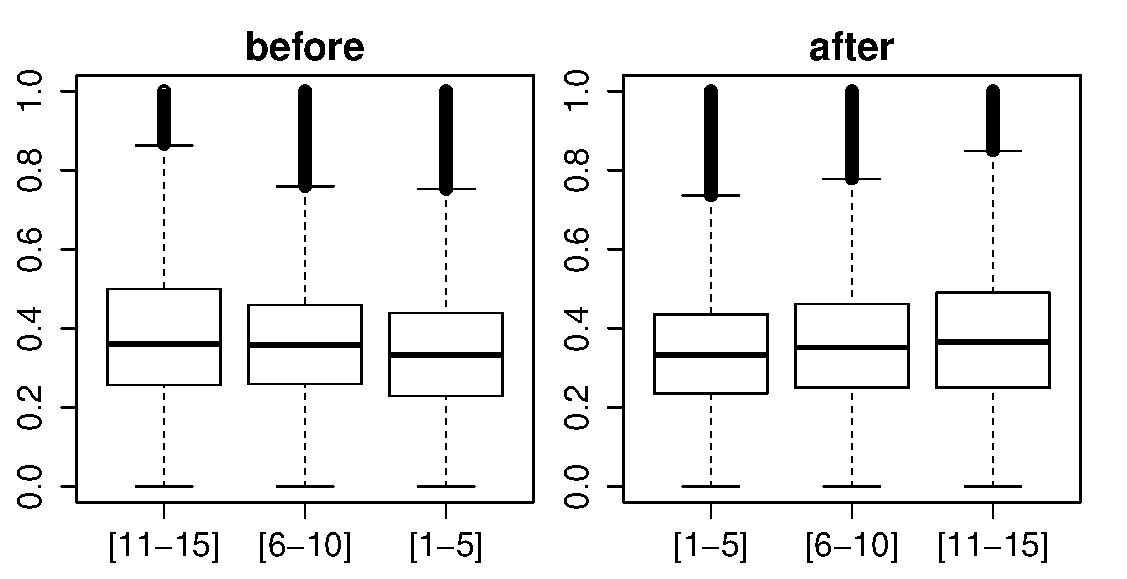
\includegraphics[width=0.9\linewidth,clip=, angle=0]{figures/ratio_all} 
\end{tabular}
\caption{Ratio of edits around the interruption. }
\label{fig:ratio_all}
\end{figure}

\begin{table}[ht!]
\renewcommand{\arraystretch}{1.3}
\caption{Effect size of the ratio of edits around the interruption.}
\label{tbl:ratio_all}
\centering
\begin{tabular}{l | p{0.7cm} | C{1.9cm} | C{1.9cm} } 
   & [1-5] & [5-10] & [11-15] \\  
  \hline
  \multicolumn{4}{c}{\textbf{before}} \\
  \hline
  mean & 0.34 &	0.37 &	0.39 \\ 
   \cline{3-4} 
  U-test & $\hookrightarrow$ & \multicolumn{2}{c}{$<$ 2.2e-16}  \\

  \cline{3-4} 
  Cohen's $d$ & $\hookrightarrow$	& \textbf{0.16} & \textbf{0.24}   \\
  \hline
  
  
  \multicolumn{4}{c}{\textbf{after}} \\
  \hline 
  mean & 0.34 &	0.37 &	0.39 \\ 
   \cline{3-4} 
  U-test & $\hookrightarrow$ & 5.67E-16 & $<$ 2.2e-16 \\  
  \cline{3-4} 
  Cohen's $d$ & $\hookrightarrow$	& \textbf{0.14} & \textbf{0.22}  \\  
\end{tabular}
\end{table}

\subsection{Patterns of Interruptions}
Given the overall activity pattern we noticed in the local analysis, we hypothesize that there are several kinds of interruptions, matching the scenarios observed in the literature: actual interruptions distracting the programmer from the task at hand, and switching tasks in case of being stuck in the current task.

We hence looked for patterns in the interruptions.  After applying clustering techniques over all the subsequences, we always found the formation of three recurrent patterns that show different effects of the interruption: neutral, positive and negative. The clustering was performed with the  K-Mediods~\cite{AMP97} technique, the Silhouette metric~\cite{RP87} to interpret and evaluate the results, the Dynamic Time Warping~\cite{KE05} as distance measure, and feature extraction techniques to reduce the dimensionality.  For this reason, we classified empirically each interruption by its local effect. 

We did so by computing Cohen's $d$ on the quantity of edits before and after the interruption. To obtain a significant effect, we need the presence of activity both before and after. Not all the interruptions meet this criteria however: some are located close to the start or the end of a session, or too close to another interruption.  In total, 53\% of the interruptions had enough data before and after the interruption and were selected for the analysis. %We used the Algorithm \ref{alg:local_effect} for the classification, and the 
Table \ref{tbl:local_effect} shows the applied thresholds and the results, accompanied with a typical example of an interruption in each category. This local analysis shows that there are indeed three well-defined groups of interruptions, with the two largest of them having clear effects on the activity in the session.

Finally, we briefly report on the edit ratios for positive and negative interruptions (see Figure~\ref{fig:ratio_rest}). We see distinct patterns as well: positive interruptions have a higher edit ratio after the interruption (in accordance with the hypothesis of a more efficient activity after having looked for missing information), while negative interruptions have a lower edit ratio after the interruption (in accordance with the hypothesis that the programmer may be rebuilding his context after an unwanted task switch).

%\begin{algorithm}[t]
 %\begin{algorithmic}[1]
   %\Require (Before edits  $B$, After edits $A$)  
   %\State $effect=`` "$
	%
	%\If{$\frac{|\bar{A} - \bar{B}|}{\sigma(A,B)} \leq 0.2$}
		%\State $effect=``neutral"$
	%\ElsIf{$\bar{A} \geq \bar{B}$}
		%\State $effect=``positive"$
	%\Else
		%\State $effect=``negative"$
    %\EndIf
    %
%\State \Return $effect$
 %\end{algorithmic} 
 %\caption{Compute the Local Effect}
 %\label{alg:local_effect}
%\end{algorithm}		

\begin{table}[ht!]
\caption{Local Effect of Interruption. }
\label{tbl:local_effect}
\centering
\begin{tabular}{p{4cm} | c}
effect & pattern \\
\hline
\textit{negative} (45\%): when the frequency of edit events decreases after the interruption (Cohen's $d < -0.2$)
	& 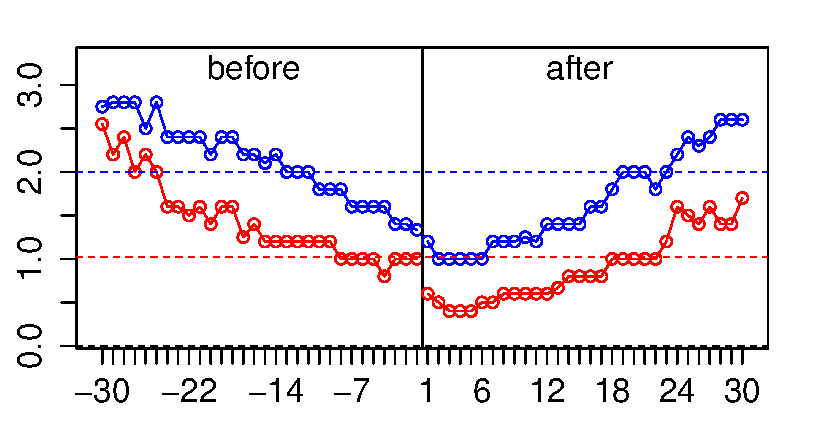
\includegraphics[valign=m,scale=0.3]{figures/neg_ints} \\
\textit{positive} (44\%): when the frequency of edit events increases after the interruption (Cohen's $d > 0.2$)
	& 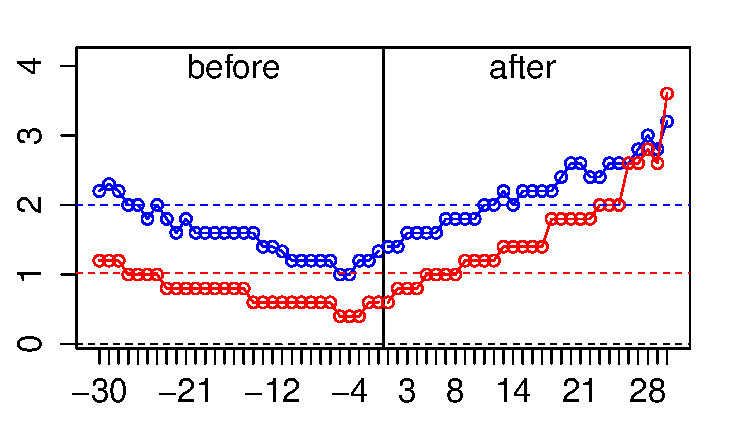
\includegraphics[valign=m,scale=0.3]{figures/pos_ints} \\
\textit{neutral} (11\%): when there is no well defined effect before or after the interruption ($abs(d) <= 0.2$)
	& 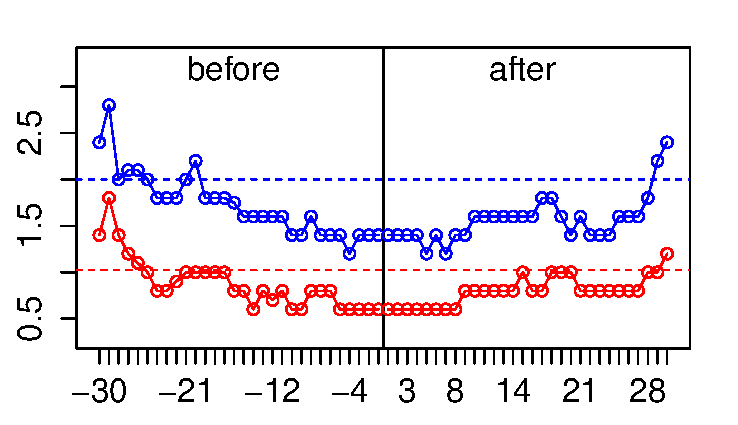
\includegraphics[valign=m,scale=0.3]{figures/neu_ints} 
\end{tabular}
\end{table}

\begin{figure}[!ht]
\centering
\begin{tabular}{c}
Positive Effect \\
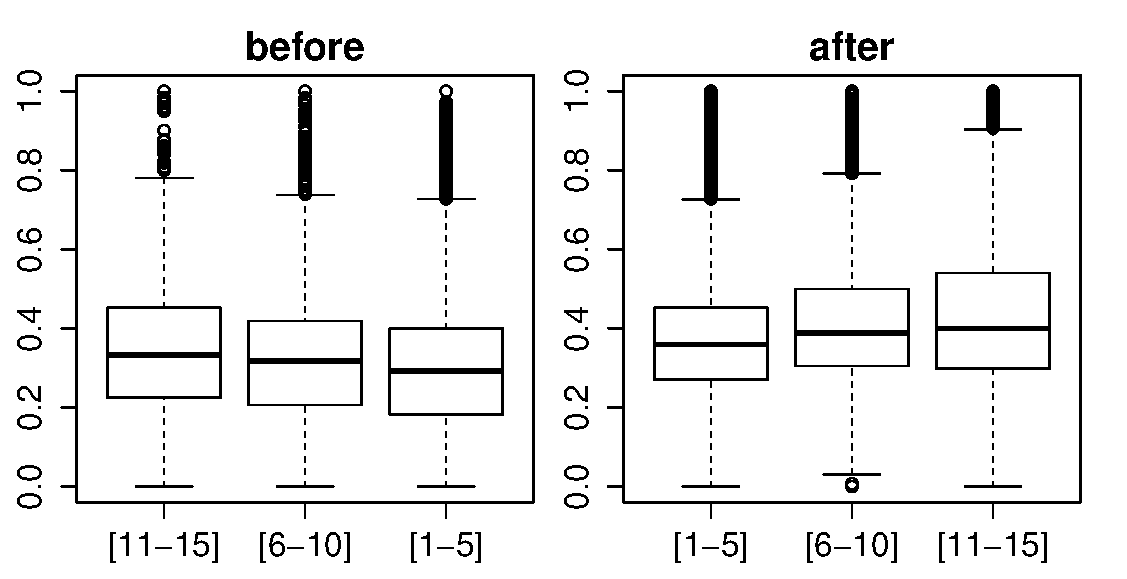
\includegraphics[width=0.9\linewidth,clip=, angle=0]{figures/ratio_pos} \\ 
\\
Negative Effect \\
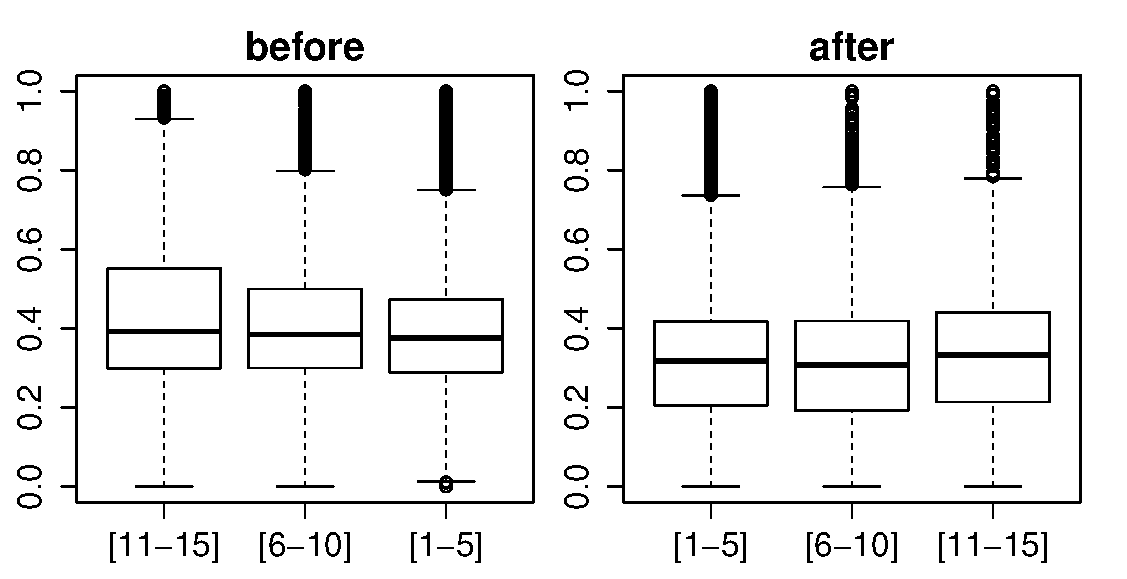
\includegraphics[width=0.9\linewidth,clip=, angle=0]{figures/ratio_neg} \\
\end{tabular}
\caption{Ratio of edits for positive and negative local effect. }
\label{fig:ratio_rest}
\end{figure}

\section{Threats to Validity}
The main threats to the validity of our study are construct validity threats due to the operational nature of the data recorded by Mylyn \cite{M14}. Most of them are mentioned above but recalled here for convenience.

The main threat to validity of the study is due to the exclusion of development session with aggregated information. We deemed that disaggregating the data as was done in other work~\cite{YR11}  was not appropriate as we do not know the exact distribution of aggregated events in time, which is very important for this study. We thus elected to filter out part of the data. We have not found evidence of bias due to this but it may still be present.

Another threat comes from the metrics we use. Our choices are limited by the data recorded by Mylyn. We believe our three indicator (edits per minute, selections per minute, and edit ratio) provide a reasonable measure of productivity (especially with the addition of edit ratio, used in other work \cite{KM06}). However we can not exclude that other indicators of productivity (such as actual changes~\cite{RL10}) may yield different results.

We defined several thresholds empirically: 8 hours of inactivity to split a session in sub-sessions, 30 minutes as the minimum duration for a session, 3 minutes for the minimum duration of a interruption and  $\geq$ 12 minutes for prolonged interruptions. We also tested with other close values and obtained similar results. However, a large variation of these thresholds might significantly alter the results. 

We acknowledge that our separation of sessions in short and long interruptions is not perfect, as it is based on the presence of at least one long interruption, and nothing more. Other factors present in the group of sessions with at least one long interruption may contribute to the observed effect (for instance, these sessions may also have more interruptions overall).

%It was very uncertain to get the best technique for disaggregating of events. Since, we unknown the temporal distribution of all the actions associated to an aggregate event. For this reason, we decided not to consider this type of traces in our analysis. However, this triggers another threat, we might have discarded main data that may alter the significance of our results. 

%Other threat is related to metrics for measuring the programmer productivity. We have analyzed the interruptions over the productive work time, the number of events by minute and the ratio of editions, which can be obtained from the interaction history. Other factors, as the code lines or the bug priority, they have not been considered in this work. One reason is because Mylyn have designed for increase the productivity in this aspects~\cite{KM06}.

The study has threats to its statistical conclusion. In particular, correlation does not necessarily implies causation: the drop in productivity may not be due to work fragmentation but to other factors (such as task difficulty). The fact that our results agree with the existing literature does help in this respect. We note that our local analysis uncovered two well-defined patterns around gaps of inactivity: ones that we hypothesize are actual interruptions (negative effect post-interruptions), and the ones that we hypothesize are more likely information-seeking activities (positive effect post-interruption). This result points to two different effects and is in need of further study. As stated in the introduction, we were careful not to conclude that every gap of activity is an actual interruption.

We used Cohen's $d$, a parametric effect size measure, as it has defined thresholds allowing easier interpretation of the results. Other effect size measures such as the common language effect size \cite{KMW92} or $A_{12}$ \cite{RRT12} may slightly alter the discussion.

This study also has threats to external validity. The gathered data corresponds to a limited group of programmers, which use both Mylyn and Eclipse regularly. The set of evolution tasks considered is a subset of the ones present on the Eclipse bug report website. It may be biased one way or another. One source of bias is the impact of Mylyn itself: Mylyn has been shown to facilitate task switching and to increase the edit ratio of its users compared to non-users. In the context of this study, we hypothesize that Mylyn could reduce the effect of work fragmentation: in other words, the observed effects may be larger for non-users. Additional studies may alleviate these threats and confirm or infirm the previous hypothesis.

%which adapted their development tasks to the platform features: Eclipse IDE $+$ Mylyn Tool. However, the bug reports did not all have associated traces and the programmers did not all submit a trace. Moreover, we used approximate measures over a sample of these data that could be analyzed. Another threat regarding data are detailed in \cite{YR11}.  The biased information that we have analyzed also is a threat to our research results. 


\section{Conclusions and Future Work}
This paper presented an empirical study on the prevalence of work fragmentation in software evolution tasks, and its relationship to developer productivity. The study was based on the Mylyn dataset of software evolution tasks, where work fragmentation is indicated by gaps of activity (interruptions) in the IDE, and productivity is measured in terms of the number of edits, selections, and the edit ratio.

We analyzed several thousands software evolution tasks, originating from several dozens of developers. Our global analysis found an inverse relationship between number and duration of interruptions and all three of our productivity indicators. These findings agree with the literature on information workers and software developers. 

A subsequent local analysis around interruptions comforted these results as the activity around interruptions was found to be lower than average. This analysis also found two well-defined patterns around interruptions: interruptions yielding a negative effects (consistent with a real-life interruption involving an expensive context switch), and interruptions with positive effects (consistent with information-seeking behavior). Further studies are necessary to expand on these findings.


\ifCLASSOPTIONcaptionsoff
  \newpage
\fi



\bibliographystyle{IEEEtran}
% argument is your BibTeX string definitions and bibliography database(s)
\bibliography{IEEEabrv,mybib}


% that's all folks
\end{document}


